\documentclass[UTF8,zihao=-4]{ctexbeamer}
\usepackage{multimedia}
\usepackage{hyperref}

\usepackage{listings}

%% 所要粘贴代码的编程语言
%\lstloadlanguages{}

%% 设置listings宏包的一些全局样式
%% 参考http://hi.baidu.com/shawpinlee/blog/item/9ec431cbae28e41cbe09e6e4.html
\lstset{
	showstringspaces=false,              %% 设定是否显示代码之间的空格符号
	numbers=left,                        %% 在左边显示行号
	numberstyle=\tiny,                   %% 设定行号字体的大小
	basicstyle=\footnotesize,                    %% 设定字体大小\tiny, \small, \Large等等
	keywordstyle=\color{blue!70}, commentstyle=\color{red!50!green!50!blue!50},
	%% 关键字高亮
	frame=shadowbox,                     %% 给代码加框
	rulesepcolor=\color{red!20!green!20!blue!20},
	escapechar=`,                        %% 中文逃逸字符,用于中英混排
	xleftmargin=2em,xrightmargin=2em, aboveskip=1em,
	breaklines,                          %% 这条命令可以让LaTeX自动将长的代码行换行排版
	extendedchars=false                  %% 这一条命令可以解决代码跨页时,章节标题,页眉等汉字不显示的问题
}

\usetheme{Madrid}
%\useoutertheme{miniframes}

\usecolortheme{orchid}
\title{基本指令及写程序思路}
\author{高星}
\institute{湖南潇湘技师学院~湖南九嶷职院}
\date{2017.09.12}
\begin{document}
    
\begin{frame}[plain]
		\maketitle
\end{frame}

\begin{frame}
\begin{columns}
\column[t]{0.3\textwidth}
\column[t]{0.7\textwidth}
\tableofcontents[hideallsubsections]
\end{columns}
\end{frame}

\section*{教学目标}

\begin{frame}{教学目标}
    \begin{columns}
        \column{.2\textwidth}
        \column{.8\textwidth}
        \begin{enumerate}
            \item 掌握手工编程的流程;
            \item 掌握基本指令;
            \item 能编写矩形凸台的程序;
            \item 掌握编程基本思路。
        \end{enumerate}
    \end{columns}
\end{frame}

\section{案例分析}
\begin{frame}{案例分析}
     \begin{columns}
        \column{.4\textwidth}
        在数控铣床或加工中心上加工如图所示的零件,试完成程序的编写,已知毛坯为 $\Phi$ 110*30。
        \column{.6\textwidth}

\begin{figure}
    \centering
    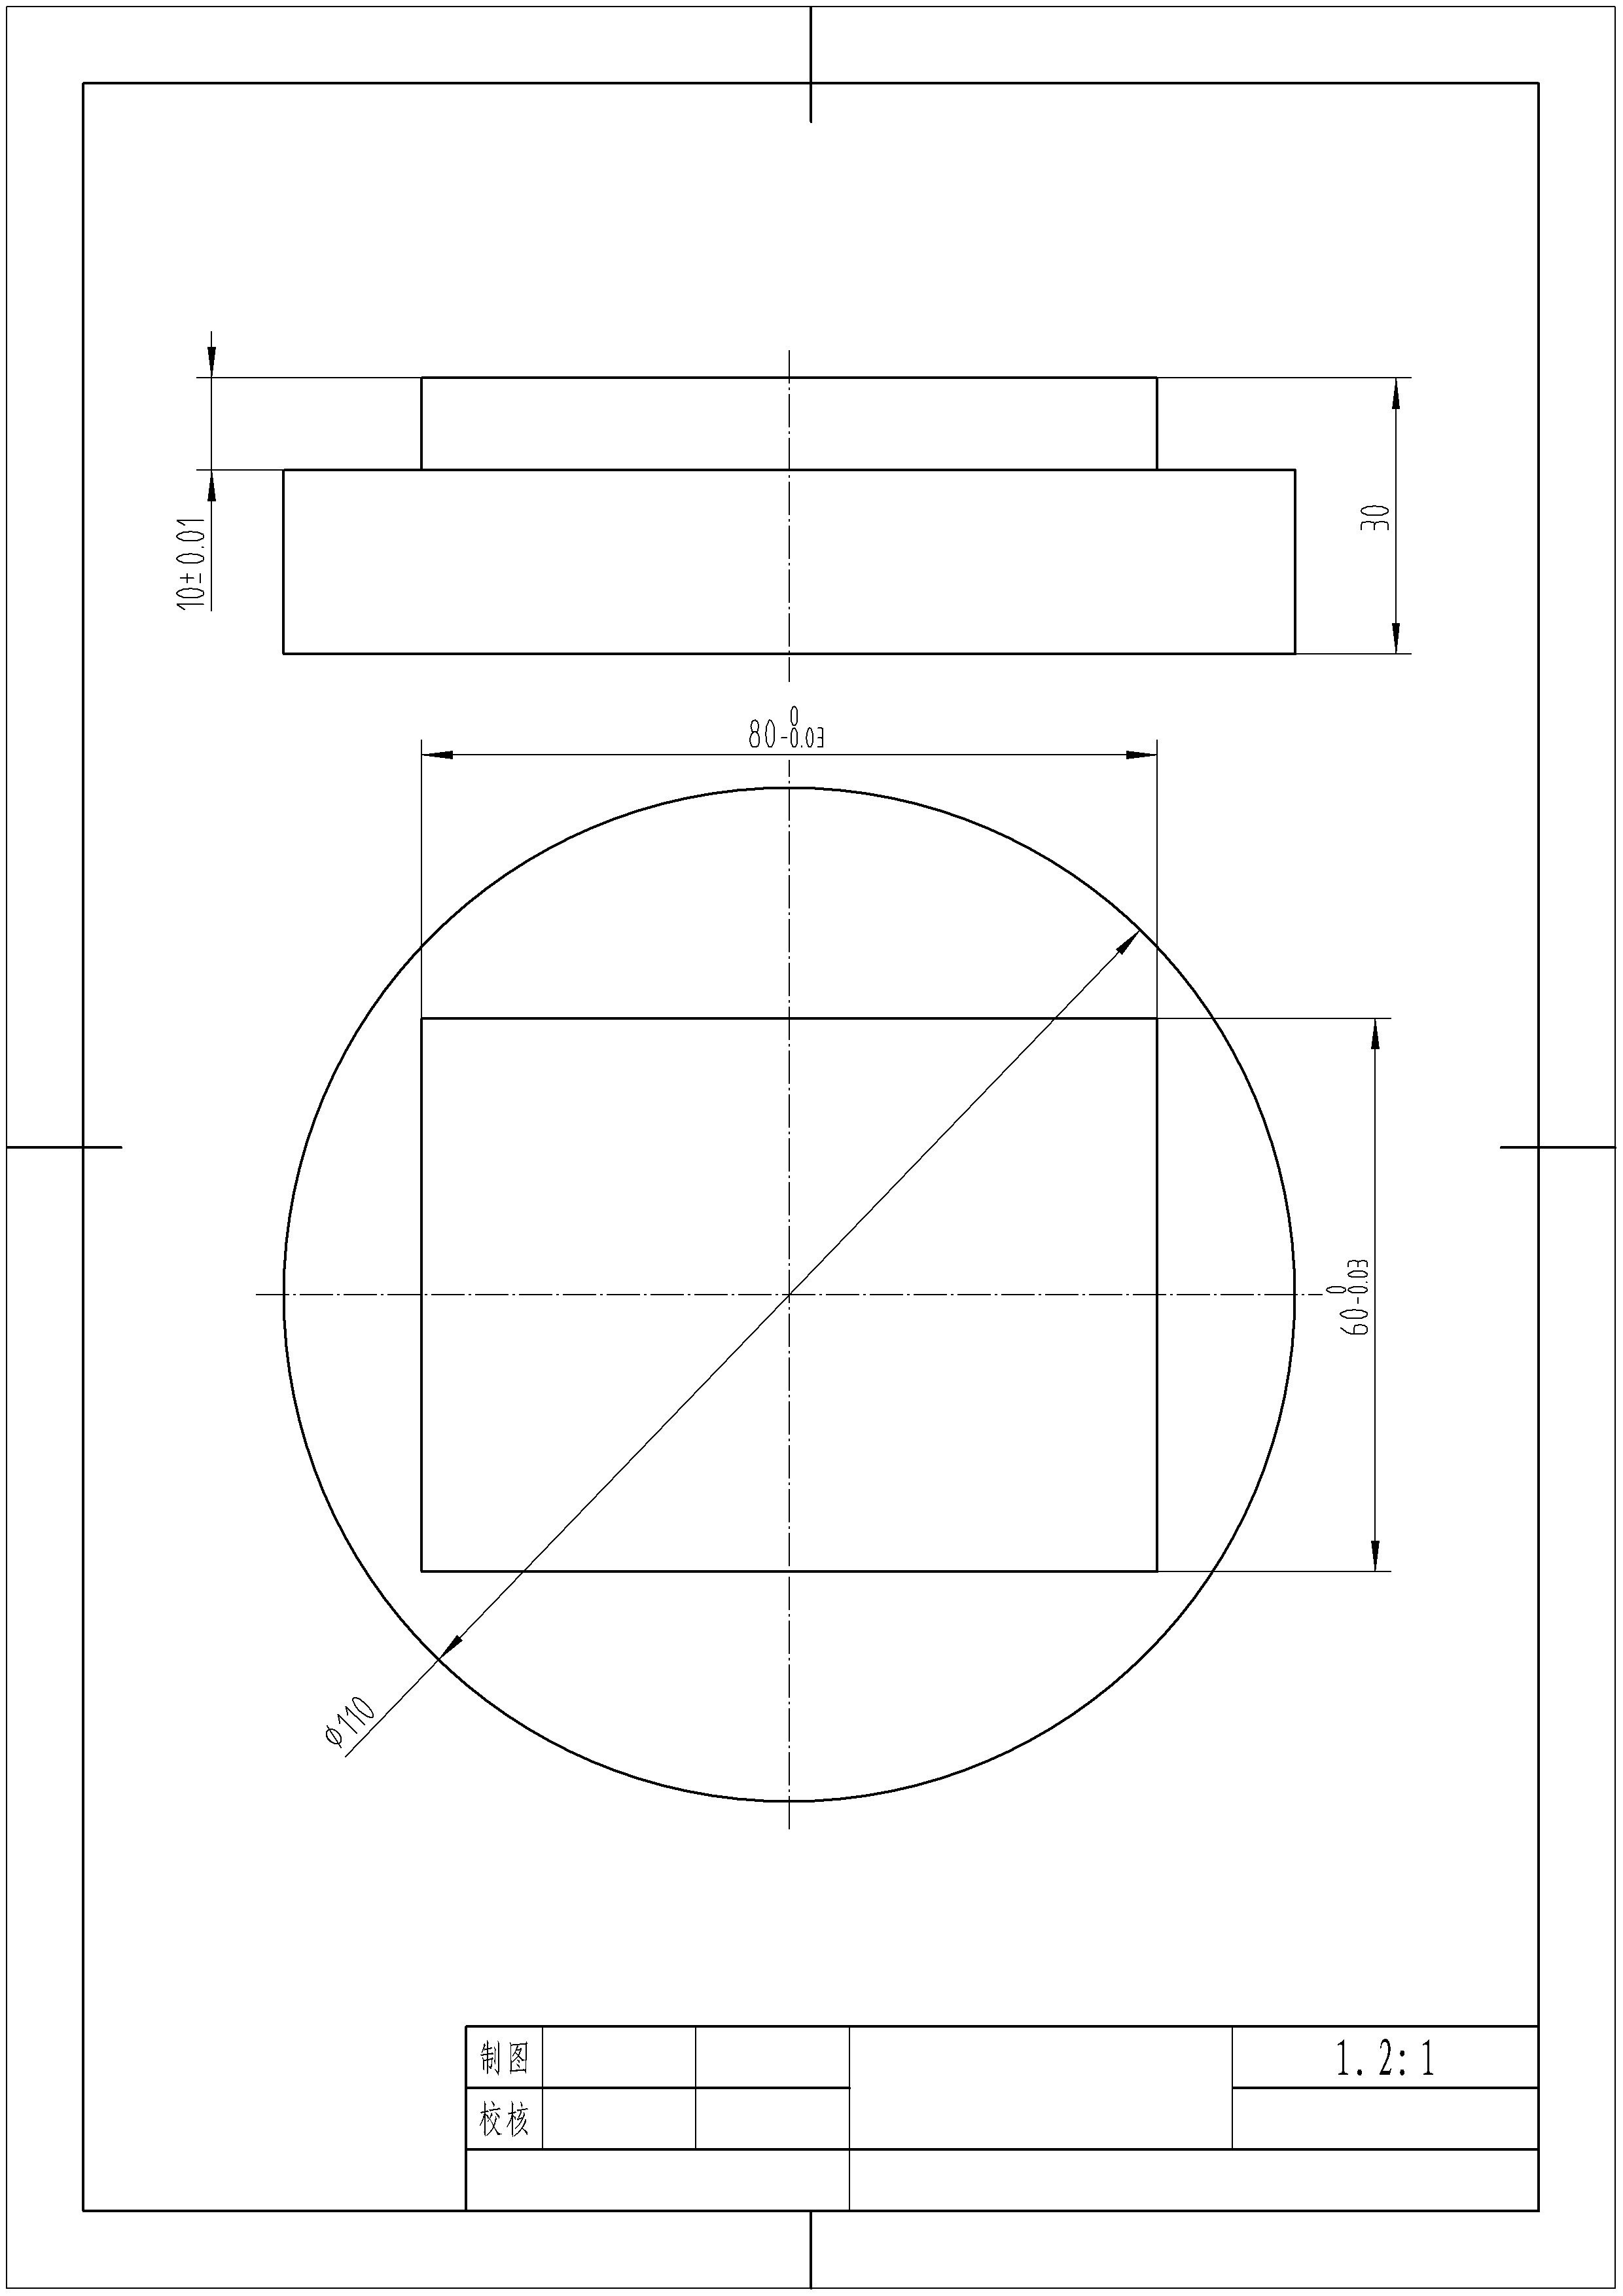
\includegraphics[width=0.8\linewidth,trim=50 150 50 100,clip]{image/3-1.jpg}
%    \caption{}
    \label{fig:3-1}
\end{figure}
    \end{columns}
\end{frame}

\begin{frame}{手工编程流程}
    \begin{columns}
        \column{.2\textwidth}
        \column{.8\textwidth}
\begin{enumerate}
    \item 图样分析;
    \item 确定加工内容;
    \item 确定装夹及工件坐标系;
    \item 确定刀具及切削用量;
    \item 确定工序及走刀路线;
    \item 计算点坐标;
    \item 编写程序单。
\end{enumerate}
    \end{columns}
\end{frame}


\section{基本指令讲解}
\subsection{程序名}
\begin{frame}{Fanuc的程序号}
    \begin{columns}
        \column{.0\textwidth}
        \column{\textwidth}
\textbf{Fanuc的程序号}

Fanuc中用程序号区分各程序,程序号由位址O跟4位数字构成;

是号,也就是说O0001号与O1号,表示同一个程序。

注意:1-7999为用户区域

8000-8999为加锁用户区域

9000-9999为厂方提供(扩展功能如O9001为换刀程序,也是加锁的)

所以用户最好别用8000-9999这些号码
    \end{columns}
\end{frame}

\subsection{安全注销指令}
\begin{frame}{安全注销指令}
    \begin{columns}
        \column{.0\textwidth}
        \column{\textwidth}
        
       1、G54-G59  选用工件坐标系,(后面讲)。
       
       2、G17-G19  加工平面选择:
       
       G17:XY平面 第一轴为X轴
       
       G18:YZ平面 第一轴为Y轴
       
       G19: ZX平面 第一轴为Z轴
       
       圆弧指令、刀具半径补偿指令、钻孔指令等使用之前有设定平面。
       
       3、G40、G49、G80 取消半径补偿、长度补偿、钻孔循环。
    \end{columns}
\end{frame}



\begin{frame}{安全注销指令}
    \begin{columns}
        \column{.0\textwidth}
        \column{\textwidth}
        
   4、G90、G91 绝对坐标编程 增量坐标编程
   
   G90指令按绝对坐标方式设定输入坐标,即移动指令终点的坐标值X、Y、Z都是以工件坐标系统坐标原点(程序零点)为基准来计算。
   
   G91指令按增量坐标方式设定输入坐标,即移动指令终点的坐标值X、Y、Z都是以始点为基准来计算,再根据终点相对于始点的方向判断正负,与坐标轴正方向一致则取正,相反取负。
   
   一般用G90,需要时采用G91,用完应立即改成G90。
    \end{columns}
\end{frame}

\subsection{主轴正反转}

\begin{frame}{主轴正反转}
    \begin{columns}
        \column{.0\textwidth}
        \column{\textwidth}
  M3 S\_ 主轴正转,其中S设定主轴转速,单位为r/min.
  
  
  注意:本学校的机床,只有加工中心可以用S,数控铣床是机械调速,S无效,Siemens上不能使用S,不然机床会一直等主轴到达设定的转速后,才接着执行后面的程序。
               
    \end{columns}
\end{frame}

\subsection{位移指令G0、G1}
\begin{frame}{位移指令G0}
    \begin{columns}
        \column{.0\textwidth}
        \column{\textwidth}
定位(G0)

G00指令使刀具以绝对或相对指令快速移到工件系统指定的位置。在绝对指令状态下,编程端点的坐标值。在相对指令状态下编程中刀具移动的距离。

[ 格式 ]

G00 IP\_\_;

IP\_\_ :
对于绝对指令,端点的坐标值。对于相对指令,是指刀具移动的距离。
    \end{columns}
\end{frame}

\begin{frame}{位移指令G0}
    \begin{columns}
        \column{.0\textwidth}
        \column{\textwidth}
        [ 说明 ]
        
        刀具轨迹通常不是一条直线。
        
        G00指令的快速移动速度是由参数No.1420由机床制造商来设定的。在实际执行G00时,刀具在单节的开始加速到预先指定的速度并在单节的结束减速。在确认到位后执行下一单节。到位的含义是指进给马达在指定的误差范围内。这个范围是由制造商在参数No.1826中设定的。
        
    \end{columns}
\end{frame}

\begin{frame}{位移指令G1}
    \begin{columns}
        \column{.0\textwidth}
        \column{\textwidth}
        刀具沿直线移动。
        
        [ 格式 ]
        
        G01 IP\_\_ F\_\_ ;
        
        IP\_\_ : 对于绝对指令,指端点的坐标,相对指令是指刀具移动的距离。
        
        F\_\_ : 刀具进给的速度(进给率)
        
    \end{columns}
\end{frame}

\begin{frame}{位移指令G1}
    \begin{columns}
        \column{.0\textwidth}
        \column{\textwidth}
        刀具沿直线移动。
        
[ 说明 ]

刀具以指定的进给率F沿直线移动到指定的位置。

进给率F有效直到赋予新值,不需要在每个单节都指定。

F码指定的进给率是沿刀具轨迹测量的。

如果不指定F值,则认为进给率为零。
        
    \end{columns}
\end{frame}

\section{零件编程}

\begin{frame}{零件编程}
    \begin{columns}
        \column{.0\textwidth}
        \column{\textwidth}
   
   
    \end{columns}
\end{frame}


\section{编写程序的基本思路}
\begin{frame}{零件编程}
    \begin{columns}
        \column{.0\textwidth}
        \column{\textwidth}
 程序初始化(安全保护)--------辅助准备(换刀,主轴启动,切削液开)--------定位到起刀点--------快速下刀--------工进下刀--------走加工轮廓--------提刀---------快速提刀到安全平面-------程序结束(换刀,主轴停止,切削液关,程序返回等)       
        
    \end{columns}
\end{frame}



\section*{课堂小结}
\begin{frame}{课堂小结}
    \begin{columns}
        \column{.2\textwidth}
        \column{.8\textwidth}
\begin{enumerate}
\item 掌握手工编程的流程;
\item 掌握基本指令;
\item 能编写矩形凸台的程序;
\item 掌握编程基本思路。
\end{enumerate}
    \end{columns}
\end{frame}

\begin{frame}{作业}
\begin{enumerate}
    \item 自定尺寸,编写加工一个矩形外形的程序?
\end{enumerate}
\end{frame}

\begin{frame}[plain]
\vfill

\centering \huge 谢谢大家!

\vfill

\flushleft \footnotesize   
~~~QQ:32731964\\
~~~TEL:18974681118\\
%~~~课件下载:\\
%~~~https://github.com/gnixoag/myworks2017/tree/master/jiaoshichengzhang

\end{frame}

\end{document} 
